\documentclass{easychithesis}

\usepackage{pdfpages}
\usepackage{csquotes}
\usepackage{nameref}
\usepackage{amsmath}    % need for subequations
\usepackage{graphicx}   % need for figures
\usepackage{changepage}
\usepackage{float}
\usepackage{caption}
\captionsetup{font={stretch=1}}
%\usepackage{verbatim}   % useful for program listings
%\usepackage{color}      % use if color is used in text
%\usepackage{subfigure}  % use for side-by-side figures
%\usepackage{hyperref}   % use for hypertext links, including those to external documents and URLs
\usepackage[numbered,framed]{docu/matlab-prettifier}

\let\ph\mlplaceholder % shorter macro
\lstMakeShortInline"

\lstset{
	style              = Matlab-editor,
	basicstyle         = \mlttfamily,
	escapechar         = ",
	mlshowsectionrules = true,
}
\begin{document}
Our goal was to construct a minimal model that is detailed enough to capture essential microscopic features of cross-linked actomyosin networks (actin filaments with asymmetric compliance, dynamic cross-links, active motors and and continuous filament turnover), but simple enough to explore, systematically, how these microscopic features control macroscopic deformation and flow. We focus on 2D networks because they capture a reasonable approximation of the quasi-2D cortical actomyosin networks that govern flow and deformation in many eukaryotic cells\cite{cellmech_flows, salbreuxbphs}, or the quasi-2D networks studied recently {\em in vitro} \cite{rheo_2D1,rheo_2D2}.




\section{Mathematical Summary of Modeling Methodology}

\subsection{Schematic Overview}
Fig. \ref{fig:model_overview} provides a schematic overview of our model's assumptions. We model each filament as an oriented elastic spring with relaxed length $l_s$. The state of a filament is defined by the positions of its endpoints $\mathbf{x_i}$ and $\mathbf{x_{i+1}}$ marking its (-) and (+) ends respectively. The index i enumerates over all endpoints of all filaments. We refer to the filament connecting endpoint i and i+1 as filament i, and we define $\mathbf{\hat{u_i}}$ to be the unit vector oriented along filament i from endpoint i to endpoint i+1.

\begin{figure}[H]
	\centering
	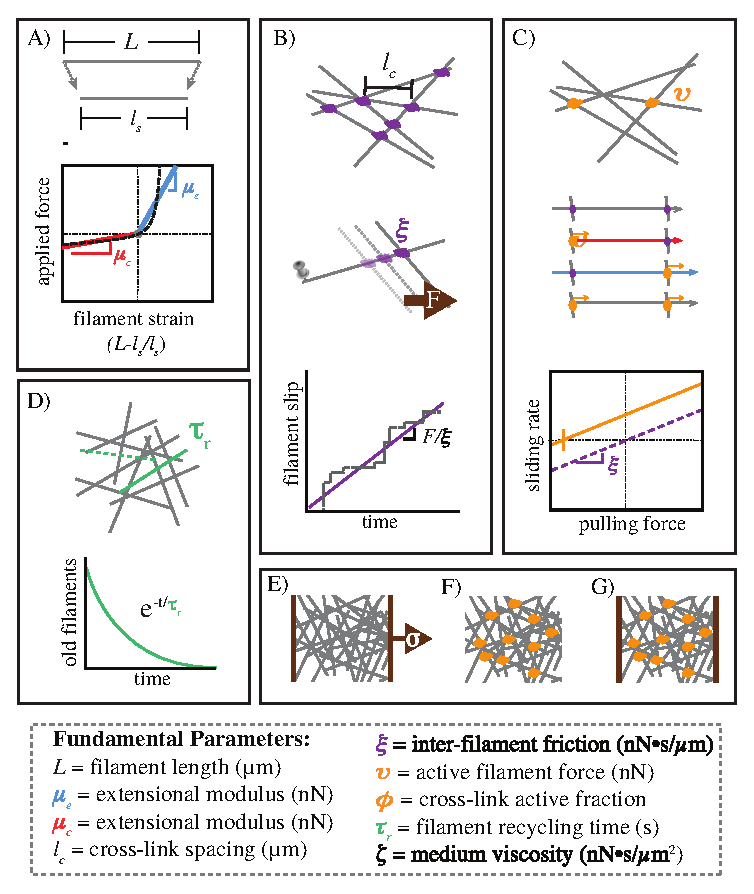
\includegraphics[width=0.8\hsize]{model/figures/Fig1}
	\caption{\label{fig:model_overview} Schematic overview of modeling framework and assumptions. \textbf{A)} Filaments are oriented linear springs that are stiffer in extension than in compression. \textbf{B)} Cross-linking occurs at all filament crossings; we represent cross link resistance as an effective drag, proportional to the relative velocity of the overlapping filaments. \textbf{C)} We represent motor activity as a linear force-velocity relationship with a fixed force at zero velocity directed towards a filament's (-) end. We implement spatial heterogeneity by imposing motor activity at a fixed fraction of filament crossover points, resulting in variation in the magnitudes of compressive vs extensile vs translational forces along individual filament segments. \textbf{D)} Whole filaments disappear at a constant rate; new filaments appear with random positions and orientations at the constant rate per unit area, such that entire network refreshes on a characteristic timescale $\tau_r$. \textbf{e-g)} Three different simulation scenarios: \textbf{E)} Passive response to uniaxial stress, \textbf{F)} Free contraction of an active network and \textbf{G)} Isometric contraction against a fixed boundary. }
\end{figure}

\subsection{Asymmetric filament compliance}
We assume (Fig. \ref{fig:model_overview}A) that local deformation of filament  i gives rise to an elastic force:

\begin{equation}
\label{eqn:spring}
\mathbf{F^{\mu}_{i,i+1}} = \mu \gamma_{i}  \mathbf{\hat{u_i}}
\end{equation}


where $ \gamma_{i} = (|\mathbf{x_{i-1}}-\mathbf{x_i}|-l_s)/l_s$ is the strain on filament i, and the elastic modulus  $\mu$ is a composite quantity that represents both filament and cross-linker compliance as in the effective medium theory of Broederz and colleagues \cite{theo_crosslinknonlinear}.  To model asymmetric filament compliance, we set $\mu = \mu_e$ if the strain is positive (extension), and $\mu = \mu_c$ if the strain is negative (compression). The total elastic force on a filament endpoint $\mathbf{i}$ can be written as:

\begin{equation}
\label{eqn:internal}
\mathbf{F^{elas}_i} =  \mathbf{F^{\mu}_{i,i+1}} - \mathbf{F^{\mu}_{i-1,i}} 
\end{equation}

In the limit of highly rigid cross-links and flexible filaments, our model approaches the pure semi-flexible filament models of \cite{theo_hlm,theo_hlm2}. In the opposite limit (nearly rigid filaments and highly flexible cross links), our model approaches that of \cite{theo_crosslinknonlinear} in small strain regimes before any nonlinear cross link stiffening. 

\subsection{Drag-like coupling between overlapping filaments}
\label{exp_drag}
Previous models represent cross-linkers as elastic connections between pairs of points on neighboring filaments that appear and disappear with either fixed or force-dependent probabilities \cite{model_taeyoon,theo_crosslinknonlinear}.  Here, we introduce a coarse-grained representation of crosslink dynamics by introducing an effective drag force that couples every pair of overlapping filaments, and which represents a molecular friction arising from the time-averaged contributions of many individual transient crosslinks (Fig. \ref{fig:model_overview}B). This coarse-grained approximation has been shown to be adequate in the case of ionic cross-linking of actin\cite{mol_fric,theo_hydroish2}, and has been used to justify simple force-velocity curves for myosin bound filaments in other contexts \cite{theo_frictionShila}. 

To implement coupling through effective drag, for any pair of overlapping filaments j and k, we write the drag force on filament j as:

\begin{equation}
\label{eqn:drag force}
\mathbf{F^{\xi}_{j,k}} = -\xi  (\mathbf{v_{j}}-\mathbf{v_{k}}) 
\end{equation}

where $\xi$ is the drag coefficient and $\mathbf{v_{j}}$, $\mathbf{v_{k}}$ are the average velocities of filaments j and k. We apportion this drag force to the two endpoints ( j, j+1) of filament j as follows: If $\mathbf{x_{j,k}}$ is the position of the filament overlap, then we assign $(1 - \mathbf{\lambda_{j,k}}) \mathbf{F^{\xi}_{j,k}}$ to endpoint j and $\mathbf{\lambda_{j,k}} \mathbf{F^{\xi}_{j,k}}$ to endpoint j+1, where $\mathbf{\lambda_{j,k}} = |\mathbf{x_{j,k}}-\mathbf{x_j}|/|\mathbf{x_{j+1}}-\mathbf{x_j}|$.

The total crosslink coupling force on endpoint i due to overlaps along filament i and i-1 can then be written:

\begin{equation}
\label{eqn: total drag couple}
\mathbf{F^{xl}_{i}} = \sum_j (1 - \mathbf{\lambda_{i,j}}) \mathbf{F^{\xi}_{i,j}} + \sum_k \mathbf{\lambda_{i-1,k}} \mathbf{F^{\xi}_{i-1,k}}
\end{equation}

where the sums are taken over all filaments j and k that overlap with filaments i and i-1 respectively.  

This model assumes a linear relation between the drag force and the velocity difference between attached filaments.   Although non-linearities can arise through force dependent detachment kinetics and/or non-linear force extension of cross-links, we assume here that these non-linear effects are of second or higher order. 

\subsection{Active coupling for motor driven filament interactions}

To add motor activity at the point of overlap between two filaments j and k ; for each filament in the pair, we impose an additional force of magnitude $\upsilon$, directed towards its (-) end (Fig. \ref{fig:model_overview}C):

\begin{equation}
\label{eqn:directedmotorforce}
\mathbf{F^{\upsilon}_{i}}=-\upsilon \mathbf{\hat{u_i}}
\end{equation}

and we impose an equal and opposite force on its overlapping partner.  We distribute these forces to filament endpoints as described above for crosslink coupling forces.  Thus, the total force on endpoint i due to motor activity can be written as:

\begin{equation}
\label{eqn:active}
\mathbf{F^{motor}_{i}} = \upsilon \sum_j (1 - \mathbf{\lambda_{i,j}}) \left (\mathbf{\hat{u_{i}}} - \mathbf{\hat{u_j}} \right ) q_{i,j}
+  \upsilon \sum_k (\mathbf{\lambda_{i-1,k}}) \left (\mathbf{\hat{u_{i-1}}} - \mathbf{\hat{u_k}} \right ) q_{i-1,k} 
\end{equation}


where j and k enumerate over all filaments that overlap with filaments i and i-1 respectively, and $q_{j,k}$ equals 0 or 1 depending on whether there is an ``active'' motor at this location. To model dispersion of motor activity, we set $q_{i,j}=1$  on a randomly selected subset of filament overlaps, such that $\bar{q}=\phi$, where $\bar{q}$ indicates the mean of $q$ (Fig. \ref{fig:model_overview}C).

\subsection{Equations of motion}

To write the full equation of motion for a network of actively and passively coupled elastic filaments, we assume the low Reynold's number limit in which inertial forces can be neglected, and we equate the sum of all forces acting on each filament endpoint to zero to obtain:

\begin{equation}
\label{eqn:syst3}
0=-l_s\zeta\mathbf{ v_i} -\mathbf{F^{xl}_i}+ \mathbf{F^{elas}_i}+\mathbf{F^{motor}_i} 
\end{equation}

where the first term represents the hydrodynamic drag on the half-filament adjoining endpoint i with respect to motion against the surrounding fluid, and $\zeta$ is the drag coefficient.

\subsection{2D network formation}

We used a mikado model approach \cite{Unterberger2014} to initialize a minimal network of overlapping unstressed linear filaments in a rectangular 2D domain. We generate individual filaments by laying down straight lines, of length L, with random position and orientation. We define the density using the average distance between cross-links along a filament, $l_c$. A simple geometrical argument can then be used to derive the number of filaments filling a domain as a function of $L$ and $l_c$ \cite{theo_hlm}.  Here, we use the approximation that the number of filaments needed to tile a rectangular domain of size $D_x \times D_y$  is $2D_xD_y/Ll_c$, and that the length density is therefore simply, $2/l_c$. 

\subsection{Modeling filament turnover}

In living cells, actin filament assembly is governed by multiple factors that control filament nucleation, branching and elongation. Likewise filament disassembly is governed by multiple factors that promote filament severing and monomer dissociation at filament ends. Here, we implement a very simple model for filament turnover in which entire filaments appear with a fixed rate per unit area, $k_{app}$ and disappear at a rate $k_{diss}\rho$, where $\rho$ is a filament density (Fig. \ref{fig:model_overview}D). With this assumption, in the absence of network deformation, the density of filaments will equilibrate to a steady state density, $k_{app}/k_{diss}$, with time constant $\tau_r = 1/k_{diss}$.   In deforming networks, the density will be set by a competition between strain thinning ($\gamma>0$) or thickening ($\gamma<0$), and density equilibration via turnover. To implement this model, at fixed time intervals $\tau_s < 0.01\cdot\tau_r$ (i.e. 1\% of the equilibration time), we selected a fraction, $\tau_s/\tau_r$, of existing filaments (i.e. less than 1\% of the total filaments) for degradation. We then generated a fixed number of new unstrained filaments $k_{app}\tau_sD_xD_y$ at random positions and orientations within the original domain.   We refer to $k_{diss}=1/\tau_r$ as the turnover rate, and to $\tau_r$ as the turnover time.


\subsection{Simulation methods}

Further details regarding our simulation approach and references to our code can be found in the Supplementary Information (\nameref{S1_Text} A.1). Briefly, equations 1-7 define a coupled system of ordinary differential equations that can be written in the form:

\begin{equation}
\mathbf{A \cdot \dot x} = \mathbf{f(x)}
\end{equation}

where $\mathbf{x}$ is a vector of filament endpoint positions, $\mathbf{\dot{x}}$ the endpoint velocities, $\mathbf{A }$ is a matrix with constant coefficients that represent crosslink coupling forces between overlapping filaments, and $\mathbf{f(x)}$ represents the active (motor) and elastic forces on filament endpoints. We smoothed all filament interactions, force fields, and constraints linearly over small regions such that the equations contained no sharp discontinuities. We numerically integrate this system of equations to find the time evolution of the positions of all filament endpoints. We generate a network of filaments with random positions and orientations as described above within a domain of size $D_x$ by $D_y$.  For all simulations, we imposed periodic boundaries in the y-dimension. To impose an extensional stress, we constrained all filament endpoints within a fixed distance $0.05\cdot D_x$ from the left edge of the domain to be non-moving, then we imposed a rightwards force on all endpoints within a distance $0.05\cdot D_x$ from the right edge of the domain.   To simulate free contraction, we removed all constraints at domain boundaries; to assess buildup and maintenance of contractile stress under isometric conditions, we used periodic boundary conditions in both $x$ and $y$ dimensions.

We measured the local velocity of the network at different positions along the axis of deformation as the mean velocity of all filaments intersecting that position; we measured the internal network stress at each axial position by summing the axial component of the tensions on all filaments intersecting that position, and dividing by network height; finally, we measured network strain rate as the average of all filament velocities divided by their positions.

We assigned biological plausible reference values for all parameters (See Table \ref{table:para}).  For individual analyses, we sampled the ranges of parameter values around these reference values shown in \nameref{S1_Table}.

\begin{table}[h]
	\centering
	\caption{Simulation parameters with reference values}
	\label{table:para}
	\begin{tabular}{|c|c|c|c|c|}
		\hline
		{\bf Parameter}             & {\bf Symbol} & {\bf Reference Value}          \\ \hline
		extensional modulus         & $\mu_e$        & $1 nN $                                               \\
		compressional modulus             & $\mu_c$     & $ 0.01 nN $                           \\
		cross-link drag coefficient & $\xi$      & $unknown $              \\
		solvent drag coefficient     & $\zeta$        & $0.0005 \frac{nN s}{\mu m^2} $      \\
		filament length             & L            & $5 \mu m$                                          \\
		cross-link spacing          & $l_c$        & $0.5 \mu m$                                         \\
		active filament force          & $\upsilon$        & $0.1 nN$                                         \\
		active cross-link fraction          & $\phi$        & $0.1<0.9$                                         \\
		domain size                 & $D_x\times D_y$            & $20\times 50 \mu m$                                 \\ \hline
	\end{tabular}
\end{table}


\section{Practical Implementation of Model Framework}

Although the prior description is useful for communicating the mathematical principles underlying my modeling framework, I also want to provide a practical explanation of the logic of the code structure.  This will help to clarify the implementation details that may be ambiguous in the above formulation and make it easier for others to approach and modify my code.

The simulation code is entirely built on top of MATLAB's ode solving functions.  Therefore, at the highest level, the entire simulation framework simply boils down to providing functions to define the ode's left and right hand side, along with the initial conditions for the system.  However, because MATLABs solvers do not allow discontinuities, discontinuous filament recycling events cannot be implemented directly in the ODE.  Effectively, it is necessary to stop the simulation solver at fixed times, reset some subset of filaments, and restart the solver with the new state every time a turnover event happens.


In the following sections, I'll walk through the code's logic in more detail, emphasizing the packages and files that modularly summarize the core functions.  First I will begin with an explanation of the command line interface used to set model parameters and deploying simulations.


\subsection{Launching simulations from the command line}



The activnet package includes a function called activnet\_gen.m, which can be used to launch simulations on any MATLAB system.  The following is the documentation of the parameters passed to this function.

\begin{verbatim}
function p = activnet_gen(zet,L,mu,kap,lc,xi,ups,phi,psi,
                          r,sig,Dx,Dy,Df,Dw,ls,lf,tinc,tfin,nonlin)
% generates an active network simulation and prints node positions
% at time steps.  Parameters are defined as follows:
%
%   zet - medium viscosity
%   L - length of the filament
%   mu - compressional modulus of the filament
%   kap - bending modulus of a filament if ls<L
%   lc - average distance between filament overlaps
%   xi - frictional resistance between two overlapping segments
%   ups - motor force at filament overlaps
%   phi - fraction of overlaps that receive a motor force
%   psi - spatial variation in motor force 
%         (if external force applied, psi sets the periodicity of 
%          force application, and psi<0 sets square wave.)
%   r - recycling rate
%   sig - applied stress in the x direction applied at Df*Dx
%         (sig<0 sets stress to be applied in y direction)
%   Dx - x-dimension of domain
%   Dy - y-dimension of domain
%   Df - position at which external force is applied
%         (if Df<0, also position in x dimension where network stops )
%   Dw - width of window in x-dimension where forces/constraints are applied
%   ls - length of filament segments
%   lf - length of force falloff at end of filament (for continuous forces)
%   tinc - time increment to return solutions 
%          (will be decreassed automatically if r is too large)
%   tfin - end time of simulation
%   nonlin - nonlinear factor by which to make filament stiffer by extension
%            (if nonlin<0, then add spacing so filaments do not reach edge)
\end{verbatim}

These parameters will be explained in more detail below, but here I'll provide a brief practical explanation for their use in setting up simulations.  The parameters \texttt{zet}, \texttt{L}, \texttt{mu}, \texttt{kap}, \texttt{lc}, \texttt{xi}, \texttt{ups}, \texttt{phi}, \texttt{r}, \texttt{sig}, \texttt{Dx}, and \texttt{Dy} are defined in the mathematical methods section above as $\zeta$, $L$, $\mu_c$, $\kappa$, $l_c$, $\xi$, $\upsilon$, $\phi$, $1/\tau_r$, $\sigma$, $D_x$, and $D_y$, respectively. The parameter \texttt{nonlin} is used to internally calculate the extensional modulus $\mu_e = \texttt{nonlin} \times \mu_c$ (i.e. if \texttt{mu} is 1 and \texttt{nonlin} is 100, then $\mu_c=1$ and $\mu_e=100$).  The parameter \texttt{psi} is used to generate a spatial gradient in internal activity or temporal periodicity if an external force is applied. The spatial gradient is linear with a maximum at the center of the domain.  The parameter \texttt{Df} defines the x-position where any external stress will be applied (i.e. stress is applied at \texttt{Df}x\texttt{Dx}).

All of these terms are positive by definition so setting certain terms negative is used to trigger certain behavior in the simulation environment:
\begin{itemize}
	\item  Setting $\texttt{mu} < 0$ enables the extensional spring to be different than the compressive.
	\item  Setting $\texttt{sig} < 0$ causes the external stress to be applied in the y direction rather than the x direction, resulting in shear stress simulations.
	\item Setting $\texttt{nonlin} < 0$ results in space being added to the edge of the domain so that no filaments intersect with the boundaries of the simulation, allowing the network to undergo unconstrained contraction.
	\item Setting $\texttt{psi} < 0$ results in oscillating positive and negative stressed being applied to the network (as opposed to a sinusoidal pattern regularly).
	\item Setting $\texttt{Df} < 0$ will cause the rightward edge of the initially generated network to end at the location where the force is applied.
\end{itemize}
   
The parameter \texttt{ls} sets the segment size of the filament.  Theoretically this segment size is very small (the size of a single actin monomer perhaps), but for computational reasons this value is set much larger.  The parameters \texttt{Dw} and \texttt{lf} set the regions over which forces will "fall off" for the domain and individual filaments, respectively.  These are just there to ensure there are no discontinuous changes in the ODE equation as filaments move around, and should be set to some smallish number, like $0.05$, but shouldn't effect the results too much overall.  Finally, \texttt{tfin} and \texttt{tinc} set the end time of the simulation and the timesteps at which to print results, respectively.  The program will automatically shrink \texttt{tinc} if the recycling rate, \texttt{r} is large enough that manual position updates must occur on timescales smaller than \texttt{tinc}.


To run a simulation with an external stress the following code could be used.

\begin{verbatim}
activnet_gen(0.001, 1, -0.01,  0,  0.8, 10, 0, 0, 0, 
             0, -0.002, 20, 4, -0.33, 0.05, 1, 0.025, 1, 10000, 100)
\end{verbatim}

To run a simulation with internal filament activity the following code could be used.

\begin{verbatim}
activnet_gen(0.001, 5, -0.01,  0,  0.3, 10, 0.1, 0.25, 0, 
             0.001, 0, 25, 25, 0.5, 0.05, 5, 0.025, 1, 10000, -100)
\end{verbatim}

Both of these have nonlinear filament extension because the third argument (\texttt{mu}) is less than 0.  The results will be printed to the MATLAB console.

The currently deployed package can also be used to launch simulations on any linux system with MATLAB 2014b or the MATLAB 2014b Compiler Runtime installed (you will need to have a \$MATLAB environt variable enabled.  Please contact your sysadmin.).  In addition, the package can be recompiled on any system running MATLAB to create a new deployment that will be (see the README.txt file for more information about deployment).  

\begin{verbatim}
./run_activnet_gen.sh $MATLAB 0.001 1 -0.01  0  0.8 10 0 0 0 0 
         -0.002 20 4 -0.33 0.05 1 0.025 1 10000 100 > output.file
\end{verbatim}






\subsection{ODE Wrapper functions }

As demonstrated above, the initialization and launch of the simulation takes place using the function activnet\_gen.m.  This function is quite simple. It just ensures proper input parameters, builds a randomized network of filaments, prints the network node positions, and then calls the function activnet.m to compute the simulation results.  From there, activnet.m takes care of pausing solvers to update filament position for recycling as well as choosing between solvers depending on the type of problem being solved.  

\subsubsection{Generating Initial Conditions}

To select the number of filaments, $N$, to generate using the input parameters, we use the approximating formula $N \approx floor(2*Dx*Dy/lc/L)$.  This formula is derived from the tiling of a $Dx \times Dy$ domain with lines of length $L$ and spacings between lines $lc$.  This diverges from the exact number of filaments needed when $L/lc$ is small, but we ignore this discrepancy because we mostly operate in the regime where $L/lc>10$.

In most cases, the network should be assembled such that the domain is filled entirely in the y dimension ($y=0$ and $y=Dy$) and filled to the left edge ($x=0$) and up to the position $x=Dp*Dx$ in the in the x-dimension.  However, in the case that the parameter \texttt{nonlin} is less than 0, we set the initial conditions such that there is an empty space of size $0.2 Dx$ and $0.2 Dy$ at the x and y boundaries.  

To keep our density the same we should adjust our calculation of $N$ above, however, in the current implementation this adjustment is not made. This is a known bug that was corrected for after-the-fact in the publication. 


\subsubsection{Choosing between active and driven simulations }

During development I noticed that there were some cases where I could skip certain sections of the computation to speed up integration of the ODEs.  In particular, when there is no internal forces generated by filament activity, the right hand side of the differential equation is easier to compute (see below).  Therefore, in any situation where internal activity is set to 0, we use the more efficient code.  The activnet.m code makes this decision by determining if there is "pulling" of filaments rather than internal force generation.  

\begin{verbatim}
pull = (isempty(nu)&&sig~=0) 
\end{verbatim}

In this case it runs a different pair of functions to compute the ODE right hand side and mass matrix (see below).

\subsubsection{Implementing Filament Recycling }

The core function of activnet.m is to serve as a wrapper for the ODE solvers mentioned above and described in greater detail below.  However, since the ODE solvers won't allow discontinuous changes to the positions of nodes, activnet.m must also carryout the task of stitching together smaller simulations and manually updating positions in between.  The code in activnet.m implements a repeated loop with calls to the underlying ode solvers. If $r>0$, a solver computes the integral between two adjacent time points in the vector of all time points to evaluate, $tt$. Then the positions are updated and the solver is used to evaluate integral for the next time interval. Logic implemented in activnet\_gen.m ensures that the timesteps are selected small enough so that there will not be too many filaments disappearing at once.

The following code chunk implements the position update for a randomly selected subset of nodes whenever the recycling rate, r, is greater than 0.  The logic implemented in activnet\_gen.m ensures that the timesteps are not so large that more than 5\% of filaments will be undergoing a discontinuous jump at any one time (i.e $r*istep*tinc <0.05$).

\begin{verbatim}
z0 = z(end,:);
if(r>0)
p = reshape(z0,[],2);
p = [mod(p(:,1),Dx),mod(p(:,2),Dy)];

i = randi(N,floor(r*istep*tinc*N)+(rand<mod(r*istep*tinc*N,1)),1);
p((i-1)*ncnt+1,:) = [Dp*Dx*rand(size(i)) Dy*rand(size(i))];
thet = rand(size(i))*2*pi;
for j = 2:ncnt
p((i-1)*ncnt+j,:) = p((i-1)*ncnt+j-1,:)+L/(ncnt-1.0)*[cos(thet) sin(thet)];
end
z0 = reshape(p,1,[]);
end
\end{verbatim}


\subsection{Overview of Numerical Integration Implementations}
As mentioned above, the solution is numerically integrated using MATLAB's built-in ODE solvers.  The ODE equation is the low-Reynolds limit of Newton's equation of motion for all the filaments.  So to implement, I simply supply an ode solver with a function to compute the right hand side of a system of differential equations ($\mathbf{f(x)}$) along with a function to compute the mass matrix ($\mathbf{A}$) that connects the derivatives on the left hand side of the ODE system.

\begin{equation}
\mathbf{A \cdot \dot x} = \mathbf{f(x)}
\end{equation}

With those two matrices the system of differential equations can then be integrated to the desired level of precision by one of MATLABs implicit ode solvers (e.g. ode15s or ode23).  In that equation, $\mathbf{x}$ simply represents the positions of filament endpoints (nodes).  Therefore $\mathbf{\dot{x}}$ is just a way to represent the velocity of every endpoint.  

The right hand side represents the forces (external or internal) driving the motion of the filaments.  The mass matrix $mathbf{A}$ represents the coupling of filaments to each other (off diagonal elements) and to the solvent in which they are embedded (diagonal elements).  Once those are provided, MATLAB's solvers take care of the integration (see MATLAB ode solver documentation for more info).


\subsubsection{Right hand sides: \textit{activnet\_act\_ode.m vs. activenet\_pull\_ode.m}}

The right hand side of the equation constitutes all the non-viscous forces in the simulation.  The most important and fundamental forces are those of the intrafilament spring mechanics.  In these simulations, filaments are represented by chains of filament segments that act as springs with particular properties.  As described above, each segment has a compressive (\texttt{mu}) and extensional ($\texttt{mu}\times\texttt{nonlin}$) spring constant that governs the motion between endpoints along the length of each filament.  There is also a bending spring constant (\texttt{kap}) which effectively tries to straighten adjoining segments if they are not already colinear.  The internal mechanical forces of all filaments in the simulation is represented in the following code snippet.

\begin{verbatim}
%% compute intrafilament forces    
l0 = L/(ncnt-1);
p = reshape(z,[],2);
p = [mod(p(:,1),Dx),mod(p(:,2),Dy)];
dp = zeros(size(p));
for n=1:ncnt:length(p)
  va_orth=[0 0];
  va = [0 0];
  la = 0;
  for i=0:ncnt-2
    vb = mydiff(p(n+i,:),p(n+i+1,:),Dx,Dy);
    lb = sqrt(vb*vb');
    gam = (lb-l0)/l0;      % extension of the segment
    f = mu*vb/lb*gam;      % longitudinal spring force
    if(mu<0)               % allow nonlinearity
      f = -f*(1+(muN-1)*double(gam>0));
    end
    dp(n+i,:) = dp(n+i,:) + f;
    dp(n+i+1,:) = dp(n+i+1,:) - f;
    
    % % below is for bending stiffness
    
    vb_orth = [-vb(2) vb(1)];
    if(i>0)
      if(va_orth*vb'>0)
        va_orth = -va_orth;
      end
      if(vb_orth*va'<0)
        vb_orth = -vb_orth;
      end
      tor = kap/l0^2*acos(max(min(va*vb'/la/lb,1),0));
      dp(n+i-1,:)=dp(n+i-1,:)+tor*va_orth/la;
      dp(n+i,:)=dp(n+i,:)-tor*va_orth/la;
      dp(n+i+1,:)=dp(n+i+1,:)+tor*vb_orth/lb;
      dp(n+i,:)=dp(n+i,:)-tor*vb_orth/lb;
    end
    va = vb;
    va_orth = vb_orth;
    la = lb;
  end
end
\end{verbatim}

The code loops over every \texttt{ncnt} nodes, which constitute the nodes of a single filament.  Next the code loops through each node of the individual filament.  First, the code evaluates the extensional force on each node given by \texttt{f = mu*vb/lb*gam} with the modification that if \texttt{mu}<0 and \texttt{gam}>0, the force constant is modified to incorporate the nonlinear extensional stiffness.  Next, the code evaluates the bending forces for adjacent segments that are not aligned using \texttt{tor = kap/l0\^2*acos(max(min(va*vb'/la/lb,1),0))}.  The \texttt{max(min(...))} is used simply to ensure that there are no aberrantly large values due to errors in evaluation of \texttt{acos} with arguments very slightly greater than 1 or less than 0.   The two vectors \texttt{va\_orth} and \texttt{vb\_orth} are calculated to direct the force orthogonal to the orientation of the filament segment.  Finally, it should be noted that a bending force is generated from both the segment behind and te segment in front of the current node of interest and that the force from these need to be assigned at both the current node and the equal and opposite force assigned at the other end of each filament.

After the basic mechanical properties of the filament are accounted for, we need to add extra forces (otherwise the simulations won't be any more interesting than just a bunch of inert springs).  What we do depends on whether the simulation is meant to represent active motors or a passive network with an external driver.  In the next two sections we cover the specifics of the force equations for both of these cases.

\subsubsection{Active ODE}

For the ODE with internal activity, we need to compute a very different force on each node.  In particular, we have to check for intersections and add forces to filaments that intersect as if they are being pulled on by an active motor at their overlap point.  To do this we will use one of the helper functions described below to return all of our overlapping lines.  After that we will step through all pairs of intersecting lines and add the appropriate force in the appropriate direction.  The following code snippet shows the process with documentation.  

\begin{verbatim}
g = lineSegmentGrid(indL,XY,Dx,Dy,l0);  % find instersecting lines

f = min(1,max(0,(g-lf/2)/(1-lf)));
for ind=1:size(g,1)
  i = g(ind,3);
  j = g(ind,4);

  vm = mydiff(p(j,:),p(j+1,:),Dx,Dy);
  lm = sqrt(vm*vm');

  edg = 1;   % this will be used to reduce the force 
			 % as it gets closer to the edge of a filament

  if(g(ind,1)<lf)
    edg = edg*g(ind,1)/lf;
  elseif((1-g(ind,1))<lf)
    edg = edg*(1-g(ind,1))/lf;
  end

  if(g(ind,2)<lf)
    edg = edg*g(ind,2)/lf;
  elseif((1-g(ind,2))<lf)
    edg = edg*(1-g(ind,2))/lf;
  end
  
  mul = 1;   % this will be used to modulate the force if
             % psi says there should be a spatial gradient
  
  if(psi>0)
    mul = double(g(ind,5)>=psi*abs(-Dx*Df));
  end
  
  tnu = nu(ceil(i/ncnt),ceil(j/ncnt))*mul;  % variation in 
											% filament force (phi)
  
  dp(i:i+1,:) = dp(i:i+1,:) + edg*tnu/lm*[vm*(1-f(ind,1));vm*f(ind,1)];
  dp(j:j+1,:) = dp(j:j+1,:) - edg*tnu/lm*[vm*(1-f(ind,2));vm*f(ind,2)];

end
\end{verbatim}

The last line shows the net force that is added to both pairs of nodes that are intersecting (\texttt{i:i+1} and \texttt{j:j+1}) with one positive and the other negative to conserve the net force to be 0.  The term \texttt{f} is calculates the distance of the overlap point between the two nearest node locations, and is used to set how much force is applied to the first vs second node.  For each iteration of the loop, the force is calculated for the \texttt{j:j+1} filament, and each interaction is stepped through twice (once with each filament in the \texttt{j:j+1} role).  The vm calculation determines the direction in which the forces will be applied.  The terms \texttt{edg} and \texttt{tnu} simply modify the applied force by scalar quantities based on closeness to the end of the filament and spatial variation in motor force intensity.



\subsubsection{Pulling ODE}

For the case of the system with an external stress, we will need to add forces at the desired location of stress, and we will need to constrain the filaments located at the edge of the domain.  The following two code snippets show these two behaviors.


\begin{verbatim}
%% add external force at centerline
if(psi>0)
val = sig*sin(psi*t);
elseif(psi<0)
val = sig*round(mod(0.5+-psi*t,1)).*(round(mod(0.55+-psi*t/2,1))-0.5)*2;
else
val = sig;
end

subp = p(:,1)>(Df-Dw)*Dx&p(:,1)<(Df+Dw)*Dx;
ff = 1-abs(p(subp,1)-Df*Dx)/Dw/Dx;
if(sig<0)
  dp(subp,1)=dp(subp,1) - Dy*val.*ff/sum(ff);
else
  dp(subp,2)=dp(subp,2) - Dy*val.*ff/sum(ff);
end
\end{verbatim}

The top section of this code calculates stress that should be applied and sets that as \texttt{val}.  If \texttt{psi} is nonzero then we are looking to have a temporally varying applied stress.  If $\texttt{psi}>0$, then we want a sinusoidally varying stress with frequency psi.  If $\texttt{psi}<0$, then we want a square wave with frequency psi.  The max stress in each case is still \texttt{sig}.

The bottom section selects the nodes that will have force added to them in \texttt{subp}.  The force to be applied to each node is not equally distributed, but instead, \texttt{ff} sets the fraction of force to be proportional to the distance to the center of the region of applied stress (set by the width \texttt{Dw}).  This distribution function is normalized so that the total amount of force is equal to the amount of force needed to set the stress to \texttt{val} (i.e. $F_{total} = \texttt{val} \times \texttt{Dy}$).  Finally the force is applied in the x direction or the y direction based on whether \texttt{sig} is greater or less than 0.


\begin{verbatim}
% % constrain edges
subp = p(:,1)<Dw*Dx;
dp(subp,:)=dp(subp,:).*repmat(4*p(subp,1)/Dw/Dx-3,1,2);

subp = p(:,1)>Dx*(1-Dw);
dp(subp,:)=dp(subp,:).*repmat(4*abs(p(subp,1)-Dx)/Dw/Dx-3,1,2);

subp = p(:,1)<3*Dx/4*Dw|p(:,1)>Dx-3*Dx/4*Dw;
dp(subp,:)=0;
\end{verbatim}

This last segment merely constrains the force at the far left and right edges of the domain to be 0 (within $0.75 \texttt{Dw}\times\texttt{Dx}$ from each edge).  There is a linear transition to \texttt{dp=0} in the remaining 25\% of the region.

It should be noted that in the "pulling" simulations, there is no need to compute the intersection of filaments.  This means that there are far fewer computations than in the active case.   I wrote two separate functions for each of the different cases simply to avoid having to perform redundant checks on the cases repeatedly (i.e. the choice is made once in the outer wrapping functions rather than having to repeatedly make the choice for which code to run on each iteration of the solver).

\subsection{Left hand side: The mysterious mass matrix}

To understand the logic of coupling filaments together by their velocities it might be helpful to look at a simple example.  Imagine that you have a single particle in some one-dimensional fluid with viscosity, $\zeta$, and with a force, $F$, acting on it.  Assuming low Reynolds limit so there is no acceleration of the particle, the equation of motion would look like the following.

\begin{equation}
\zeta\dot{x}=F
\end{equation}

Now assume you have two particles in that fluid, but (for now) we assume the particles can't interact in any way.  Therefore, we can express the equation of motion for both particles pretty simply with the following equation.

\begin{equation}
\zeta\mathbf{\dot{x}}=\mathbf{F}
\end{equation}

Obviously, all we did was replace the scalars with vectors.  To make things a little neater we could replace the scalar $\zeta$ with a so called "mass matrix" that would simply look like the following matrix.

\begin{equation}
\mathbf{A} = \begin{bmatrix} \zeta & 0 \\ 0 & \zeta \end{bmatrix}
\end{equation}

Now, if we had some drag-like coupling between the velocities of our two particles with a drag coefficient, $\xi$, we could simply add a term to the off diagonal.

\begin{equation}
\mathbf{A} = \begin{bmatrix} \zeta & -\xi \\ -\xi & \zeta \end{bmatrix}
\end{equation}

And carrying out our math we can see that this just gives a frictional coupling between the two particles.

\begin{equation}
\begin{array}{lcl} \zeta v_1 - \xi v_2  & = & F_1 \\ \zeta v_2 - \xi v_1 & = & F_2 \end{array}
\end{equation}

This is the entire logic behind the construction of the activnet\_mass.m function.  After finding which filament segments are overlapping, I simply add off-diagonal terms to the mass matrix that couple the nodes of those filament segments together.

Similar to the previous section, there are computational efficiencies to be gained in computing the mass matrix, $\mathbf{A}$, if the system is being driven externally (as opposed to being driven by internal activity).  

\subsubsection{\textit{activnet\_mass.m vs. activenet\_mass\_sp.m}}
When we are constraining filaments to remain motionless we run into one little problem with our mass matrix formulation as presented thus far.  Essentially, the right hand side of the equation is being set to 0, but the left hand side still has cross terms .  To remedy this, in the case where an external stress is applied, I need to manually decouple filaments that lie along the $x=0$ boundary of the domain.  This is carried out in activenet\_mass\_sp.m, but it is not implemented in activenet\_mass.m because that code only runs in the case where there is internal activity of the filaments and no external constraints.

Additionally, in activenet\_mass\_sp.m, I utilize a sparse matrix for reasons that I honestly don't exactly remember.  I assume that I found in that condition I could get some kind of marginal speedup by using a sparse matrix instead of the full matrix.


\subsection{Line intersection \textit{helper} Functions}
There are a series of helper functions that are called to aid in the calculations of filament intersections.  Yu can analyze the code directly for more detail but briefly, the lineSegmentIntersect.m implementation manually computes the intersection between all pairs of segments while lineSegmentGrid.m first bins lines into grids before testing intersection just on those in the bin.  I saw a significant improvement when I moved to lineSegmentGrid even though asymptotically they both perform worst case $O(n^2)$, which I believe is due to the uniformity of the line segment distribution.  Some mathematician might be able to prove that.  It is interesting to note that the classical best-case line scanning algorithm (i.e. sweep line) is $O(nlogn)$.

\subsection{Visualization code}
In the analysis package, I have included some code called netplot\_str.m to aid with visualizing the output of the simulations.  This code opens the output file and an accompanying script file to get the parameters passed to the function.  The code then goes on to render all the lines in a MATLAB plot.  It could e modified easily to render the output in whatever format you may need.  However, it is important to note that you need the input parameters to correctly associate output nodes to their correct filament.

%\bibliography{active/slippage,active/active,edeals/bibliography}
%\bibliographystyle{plain}

\end{document}
